\documentclass[11pt,a4paper]{article}

\usepackage[margin=2.5cm]{geometry}
\usepackage{amsmath,amssymb,amsfonts}
\usepackage{mathtools}
\usepackage{booktabs}
\usepackage{graphicx}
\usepackage{xcolor}
\usepackage{hyperref}
\usepackage{microtype}
\usepackage{enumitem}
\usepackage{caption}
\usepackage{subcaption}

\hypersetup{
  colorlinks=true,
  linkcolor=blue!60!black,
  citecolor=blue!60!black,
  urlcolor=blue!60!black,
  pdftitle={Cogenetic Minkowski Functional (CMF)},
  pdfauthor={Morgan Petrik, Militant.AI}
}

\newcommand{\docversion}{1.0.0}
\newcommand{\docdoi}{10.5281/zenodo.20808466}

\title{%
  \textbf{Cogenetic Minkowski Functional}\\[0.4em]
  \large Version \docversion
}
\author{%
  Morgan Petrik\\[0.35em]
  {\itshape Militant.AI}%
}
\date{%
  23 June 2026\\[0.6em]
  {\small DOI:~\href{https://doi.org/\docdoi}{\docdoi}}%
}

\newcommand{\M}{\mathcal{M}}
\newcommand{\Ph}{\Phi}

\begin{document}
\maketitle

\begin{abstract}
Following \emph{Cogenesis}~\cite{petrik2026cogenesis}: relation is prior to being; spacetime, metrics, and measurement are \textbf{projections} of a deeper process-field, not primitives. Minkowski's fusion of time with space into a $(3{+}1)$ manifold was a \textbf{modern calculus utilitarian simplification}---an accounting convention for Lorentz covariance and perturbation theory. Standard practice \textbf{reified} that convention into ``spacetime.'' That is the error: fundamentalising time as a fourth dimension on par with space, and treating $(\M,\eta)$ as the relational dynamics of reality rather than as projected bookkeeping.

\textbf{Cogenetic Minkowski Functional (CMF)} is the Minkowski-stage observation functional in that residual-aware framework. It keeps the calculus machinery---flat $\eta$, light cones, variational methods---while refusing the reification. $\eta$ is the \textbf{zeroth-order low-residual projection}, not ground truth. Environment enters as \textbf{$C$}---the environmental density gradient along the observer's throughline. \textbf{Process time} $t$ indexes resolution \textbf{$R(t)$}---not a rename of $t$ as resolution, but the map $t \mapsto R(t)$ at which the functional is evaluated and sharpens as the process runs.

CMF is a \textbf{refinement algorithm} on the \textbf{projection calculus}---against the \textbf{process calculus} beneath it: project, measure residual, recover flat $\eta$ only where $|r_{C,R}|$ is negligible. Flat Minkowski remains \emph{usable} when the utilitarian simplification suffices---when ignoring $C$ and $R(t)$ is adequate for the accounting task, not because spacetime is true.

This document specifies the construction, contrasts it with the bolted-on input pattern of standard practice, and separates what Minkowski \emph{stipulates} from what CMF \emph{determines} at each process time and \emph{predicts} over the running observation. A reference implementation with a satellite point-detector example is included.
\end{abstract}

\section{Problem statement}

\subsection{What the Minkowski calculus is for}

On $\M = \mathbb{R}^{3,1}$ with metric $\eta_{\mu\nu} = \mathrm{diag}(-c^2,1,1,1)$, the interval
\begin{equation}
  ds^2 = \eta_{\mu\nu}\, dx^\mu dx^\nu
\end{equation}
is a \textbf{utilitarian simplification}: a flat stage for special relativity, QFT regularisation, and linearised gravity. The apparatus is proven and cheap to use. None of that makes $(\M,\eta)$ a reification of relational reality.

\subsection{Where reification goes wrong}

Minkowski's $(3{+}1)$ fusion was an accounting hack---time promoted to a fourth coordinate so Lorentz transformations act linearly on a single object. Standard practice then:
\begin{enumerate}[noitemsep]
  \item fixes a functional early---e.g.\ $F[\Ph] = \int |\Ph|^2\, d\mu$, an action $S[\Ph]$, or a Green's function;
  \item treats \emph{environment} and \emph{process} as \emph{external inputs} bolted on afterward;
  \item treats \emph{events} as primitive points on $\M$;
  \item identifies this \emph{calculus projection} with \emph{physical reality}.
\end{enumerate}

Spacetime as primitive is a category error. It hides what any finite observation already carries: observer location, environment along the throughline, running process time $t$ and resolution $R(t)$, and the residual lost when a continuous field is projected to an observable. CMF makes these explicit \emph{inside} the functional, not as afterthoughts.

\subsection{Design principle}
\label{sec:design-principle}

\textbf{Process calculus} carries the relational dynamics: observer throughline, environment $C$, process time $t$, resolution $R(t)$, and the residual $r_{C,R}$ lost on projection.

\textbf{Projection calculus} is the utilitarian simplification Minkowski built from that dynamics: flat $(\M,\eta)$, intervals, Lorentz covariance, variational machinery~\cite{petrik2026cogenesis}. It is bookkeeping that converges when $|r_{C,R}|$ is negligible---not a second ontology.

CMF uses both without collapsing them:
\begin{equation}
  \boxed{\;\text{Process calculus is primary; $(\M,\eta)$ is projection calculus, not relational reality.}\;}
  \label{eq:zeroth-order}
\end{equation}

\section{Formal construction}

\subsection{Base stage}

Retain the Minkowski background
\begin{equation}
  \M = \mathbb{R}^{3,1}, \qquad \eta_{\mu\nu} = \mathrm{diag}(-c^2,1,1,1)
\end{equation}
as the working stage of \textbf{projection calculus} (\S\ref{sec:design-principle})---not \textbf{process calculus}.

\subsection{Process field}

Introduce a smooth process field
\begin{equation}
  \Ph : \M \to V
\end{equation}
where $V$ is a finite-dimensional vector space (scalar, spinor, or internal coherence space).

\subsection{Context \texorpdfstring{$C$}{C}}

$C$ is the declared local condition under which process becomes distinguishable:
\begin{equation}
  C = (U,\, e^\mu_a,\, A,\, B,\, I,\, E,\, G)
\end{equation}

\begin{table}[h]
  \centering
  \caption{Components of context $C$.}
  \label{tab:context}
  \begin{tabular}{@{}ll@{}}
    \toprule
    Component & Meaning \\
    \midrule
    $U \subset \M$ & Region of distinguishability \\
    $e^\mu_a$ & Observer / tetrad frame \\
    $A$ & Apparatus or observation functional \\
    $B$ & Boundary / initial data \\
    $I$ & Preparation / input condition \\
    $E$ & Environmental coupling \\
    $G$ & Gauge / coordinate convention \\
    \bottomrule
  \end{tabular}
\end{table}

\paragraph{Operational form (primary).}
For a point detector on a throughline---e.g.\ a satellite sighting a surface target---$C$ is the environmental density gradient along the observer ray:
\begin{equation}
  C(x) = \hat{n} \cdot \nabla \rho_{\mathrm{env}}(x)
  \label{eq:context-gradient}
\end{equation}
where $\rho_{\mathrm{env}}$ is environmental density (atmosphere, medium, noise background) and $\hat{n}$ is the unit vector from observer to target. $C$ is not metadata bolted onto a fixed functional; it shapes the map itself.

\subsection{Process time and resolution \texorpdfstring{$R(t)$}{R(t)}}

In the core formalism, $R$ denotes \textbf{resolution}---finite distinction capacity---not calendar time. CMF does \emph{not} identify $R$ with coordinate time $t$. Instead, \textbf{process time} $t$ is the running index of the observation process, and $t$ maps to an evolving resolution state:
\begin{equation}
  t \;\longmapsto\; R(t) = \bigl(\ell(t),\, \tau(t),\, \Lambda(t),\, \epsilon(t),\, \Sigma(t)\bigr)
  \label{eq:R-of-t}
\end{equation}
At each $t$, the map uses $R(t)$ inside $\Pi_{C,R(t)}$, $|r_{C,R(t)}|$, and $O(C,R(t))$. Early $t$: coarse $(\ell,\tau,\Lambda)$. As the process runs, $R(t)$ sharpens. $t$ is \emph{when} the observation is happening; $R(t)$ is \emph{how sharply} it can distinguish at that moment.

\begin{table}[h]
  \centering
  \caption{Components of resolution $R(t)$ at process time $t$.}
  \label{tab:resolution}
  \begin{tabular}{@{}ll@{}}
    \toprule
    Component & Meaning \\
    \midrule
    $\ell(t)$ & Spatial resolution \\
    $\tau(t)$ & Temporal sampling window \\
    $\Lambda(t)$ & Bandwidth cutoff \\
    $\epsilon(t)$ & Distinction tolerance \\
    $\Sigma(t)$ & Noise / error covariance \\
    \bottomrule
  \end{tabular}
\end{table}

$(\ell,\tau,\Lambda)$ improve as $t$ advances; $(\epsilon,\Sigma)$ carry apparatus and environmental limits at each $t$. Subscripts on $C,R$ mean evaluation at the resolution state $R(t)$ reached at process time $t$.

\subsection{Projection operator}

\begin{equation}
  (\Pi_{C,R}\Ph)(x) = \int_U K_{C,R}(x,y)\, A_C[\Ph](y)\, d\mu_\eta(y)
  \label{eq:projection}
\end{equation}
where $K_{C,R}$ is a smooth sampling kernel determined by $(\ell,\tau,\Lambda,\epsilon,\Sigma)$ and weighted by context $C$ along the throughline, and $A_C$ is the apparatus functional.

\subsection{Residual}

\begin{equation}
  r_{C,R}[\Ph] = \Ph - \iota_C \Pi_{C,R}\Ph
  \label{eq:residual}
\end{equation}
where $\iota_C$ embeds the projected observable back into the modelling space. The residual is \textbf{measurable}:
\begin{equation}
  |r_{C,R}|^2 = \int_U \langle r_{C,R}(x), r_{C,R}(x) \rangle\, d\mu_\eta(x)
\end{equation}
This is exactly the information a pure Minkowski projection suppresses.

\section{Effective metric and interval}

\subsection{Metric family}

\begin{equation}
  g^{C,R}_{\mu\nu} = \eta_{\mu\nu} + h^{C,R}_{\mu\nu}[\Pi_{C,R}\Ph,\, r_{C,R}]
  \label{eq:metric}
\end{equation}

First-order calculus-compatible correction:
\begin{equation}
  h^{C,R}_{\mu\nu} = a\,\partial_\mu \rho_{C,R}\,\partial_\nu \rho_{C,R}
  + b\, J^r_\mu J^r_\nu + c\, \Xi^{C,R}_{\mu\nu}
  \label{eq:h-correction}
\end{equation}
where
\begin{equation}
  \rho_{C,R} = |\Pi_{C,R}\Ph|^2, \qquad J^r_\mu = \partial_\mu |r_{C,R}|^2
\end{equation}
and $\Xi^{C,R}_{\mu\nu}$ is a fragmentation / decoherence tensor from projected gradients and noise.

\subsection{Interval}

\begin{equation}
  ds^2_{C,R} = g^{C,R}_{\mu\nu}\, dx^\mu dx^\nu
  = \eta_{\mu\nu}\, dx^\mu dx^\nu + h^{C,R}_{\mu\nu}\, dx^\mu dx^\nu
\end{equation}

\subsection{Minkowski recovery condition}

Minkowski is recovered when
\begin{equation}
  \Pi_{C,R}\Ph \text{ is uniform}, \qquad r_{C,R} \to 0, \qquad \Xi^{C,R}_{\mu\nu} \to 0.
\end{equation}
Equivalently: \textbf{flat $\eta$ is the $(C,R)$-low-residual limit of the projected functional---a simplification that converges, not a discovered spacetime.}

\section{The refinement algorithm}

CMF is not parameter tuning. It is a \textbf{process}:
\begin{enumerate}
  \item \textbf{Declare $C$}---fix the environment and observer throughline (e.g.\ satellite position, target, $\rho_{\mathrm{env}}$).
  \item \textbf{Set process time $t$}---resolve $R(t)=(\ell(t),\tau(t),\Lambda(t),\epsilon(t),\Sigma(t))$ and evaluate at this moment of observation.
  \item \textbf{Project}---compute $\Pi_{C,R(t)}\Ph$.
  \item \textbf{Measure residual}---compute $|r_{C,R(t)}|^2$.
  \item \textbf{Advance process time}---as $t$ increases, $R(t)$ sharpens and the functional refines.
  \item \textbf{Recover Minkowski}---when residual falls below tolerance, flat geometry is a valid zeroth-order description.
\end{enumerate}

\begin{equation}
  \boxed{
  (\M,\eta) \;\longrightarrow\; (\M,\eta,\Ph,\Pi_{C,R},r_{C,R},g^{C,R})
  }
\end{equation}

\section{Observers and events}

Events are \textbf{not} primitive points. An observation is
\begin{equation}
  O_i(C,R) = \int_U K^i_{C,R}(x)\, F_i(\Ph,\partial\Ph,g^{C,R})\, d\mu_{g^{C,R}} + \epsilon_i
  \label{eq:observer}
\end{equation}
a finite-resolution projection of field-process into an observable, with sampling noise $\epsilon_i$.

\begin{table}[h]
  \centering
  \caption{Standard practice vs.\ CMF.}
  \label{tab:contrast}
  \begin{tabular}{@{}p{0.42\linewidth}p{0.48\linewidth}@{}}
    \toprule
    Standard & CMF \\
    \midrule
    Fixed $F[\Ph]$ & Process functional $F[\Ph; C, R(t)]$ \\
    $C$, $R$ bolted on as inputs & $C$, $R$ inside the map \\
    Same answer at all times & Functional sharpens with process time \\
    Event $=$ point on $\M$ & Event $=$ kernel projection \\
    \bottomrule
  \end{tabular}
\end{table}

\section{Dynamics (optional extension)}

Field dynamics remain calculus-based. Action:
\begin{equation}
  S[\Ph] = \int_\M \left[
    \tfrac{1}{2}\, \eta^{\mu\nu} \langle \partial_\mu \Ph, \partial_\nu \Ph \rangle
    - V(\rho_{C,R},\Xi) + \tfrac{\alpha}{2}\, |r_{C,R}|^2
  \right] d^4x
\end{equation}

Euler--Lagrange equations yield PDEs with residual source terms:
\begin{equation}
  \Box_\eta \Ph + \frac{\partial V}{\partial \Ph} = J_r
\end{equation}
The residual source $J_r$ is what old Minkowski projection would drop.

\section{When the utilitarian simplification suffices}

\begin{quote}
  \textbf{Use flat $\eta$ when the accounting simplification is adequate for the task---not because spacetime is true.}
\end{quote}

\begin{table}[h]
  \centering
  \caption{When flat $\eta$ suffices vs.\ when to carry CMF.}
  \label{tab:when}
  \begin{tabular}{@{}ll@{}}
    \toprule
    Situation & Recommendation \\
    \midrule
    Back-of-envelope kinematics & Flat $\eta$---simplification suffices \\
    Lab frame, long integration, buried error budget & Often suffices \\
    Satellite line-of-sight through density gradient & Carry CMF \\
    Early integration, targeting decisions & Carry CMF \\
    Residual-dominated regime & Do not reify $\eta$ as ontology \\
    \bottomrule
  \end{tabular}
\end{table}

Flat Minkowski is a \textbf{utilitarian simplification}, not relational reality. CMF adds no overhead when the simplification is adequate: set $h \to 0$ and recover $\eta$. Carry $C$ and $R(t)$ when the accounting task requires what the projection suppresses.

\section{Stipulations vs.\ determination}

CMF is a \textbf{cogenetic} projection formalism~\cite{petrik2026cogenesis}: observables co-emerge with context and process time. Judging it against general relativity or quantum field theory as a ``correction'' is the wrong frame---those theories already presuppose flat $\eta$ as stage~\cite{petrik2025omqg}. The correct comparison is \textbf{CMF vs.\ standard Minkowski practice}.

The distinction is methodological, not a claim that CMF never predicts anything:
\begin{itemize}[noitemsep]
  \item \textbf{Minkowski stipulates}---at a given setup, standard practice \emph{fixes} $|r_{C,R}|=0$, $g=\eta$, and a functional with no $R$-map inside it. These are prior commitments of the calculus stage, not outputs of an observation process.
  \item \textbf{CMF determines}---at each process time $t$, the map resolves $R(t)$ and computes $|r_{C,R(t)}|$, $g^{C,R(t)}=\eta+h$, and $O(C,R(t))$ from $(\Ph,C,t)$ via project $\to$ measure residual $\to$ evaluate observer \eqref{eq:observer}.
  \item \textbf{CMF predicts}---over process time, the formalism claims refinement behaviour: falling residual, sharpening $O(C,R)$, and a bolted-on $F[\Ph]$ that cannot track any of it.
\end{itemize}

\subsection{What Minkowski stipulates}

\begin{table}[h]
  \centering
  \caption{Values fixed by standard Minkowski practice before the observation process runs.}
  \label{tab:stipulations}
  \begin{tabular}{@{}ll@{}}
    \toprule
    Stipulation & Value \\
    \midrule
    Residual & $|r_{C,R}| = 0$ \\
    Metric & $g^{\mu\nu} = \eta^{\mu\nu}$ \\
    Interval correction & $|g_{xx}-\eta_{xx}| = 0$ \\
    Functional & $F[\Ph]$ with no $R$-dependence \\
    Over process time & No change---$C$ and $R$ bolted on externally \\
    \bottomrule
  \end{tabular}
\end{table}

These are utilitarian defaults---often adequate. They are not computed from the throughline environment or the running observation.

\subsection{What CMF determines at each \texorpdfstring{$R$}{R}}

At every process time, CMF \textbf{derives} quantities Minkowski practice cannot represent:
\begin{itemize}[noitemsep]
  \item \textbf{Residual} $|r_{C,R}|^2 = |\Ph - \iota_C \Pi_{C,R}\Ph|^2$ along the throughline.
  \item \textbf{Metric correction} $h[\Pi\Ph,r]$ and $g^{C,R}=\eta+h$; in vacuum $g_{xx}=1$, where $|C|>0$ and the process field has structure, $|g_{xx}-\eta_{xx}|$ is generally nonzero.
  \item \textbf{Observer reading} $O(C,R)$ from \eqref{eq:observer}---a kernel projection of $\rho_{C,R}=|\Pi_{C,R}\Ph|^2$ under $d\mu_{g^{C,R}}$, not raw $|\Ph|^2$ at a point.
\end{itemize}

\paragraph{What we do \emph{not} compare.}
CMF does \textbf{not} claim that $O(C,R)$ converges to raw $|\Ph|^2$ at a point. Comparing $O(C,R)$ to $|\Ph(0,0)|^2$ is the wrong metric. The correct comparison is \textbf{stipulation vs.\ determination}: what Minkowski \emph{fixes in advance} versus what CMF \emph{computes from the map} at each $R$.

\subsection{What CMF predicts over \texorpdfstring{$R$}{R}}

\begin{table}[h]
  \centering
  \caption{Process behaviour: stipulation vs.\ determination vs.\ prediction.}
  \label{tab:predictions}
  \begin{tabular}{@{}p{0.42\linewidth}p{0.48\linewidth}@{}}
    \toprule
    Minkowski (stipulates) & CMF (determines / predicts) \\
    \midrule
    $|r_{C,R}| = 0$ always & determines $|r_{C,R}|^2$; coarse-to-fine refinement drives it down \\
    $O$ independent of $R$ & determines $O(C,R(t))$; predicts sharpening with $R$ \\
    $g^{\mu\nu} = \eta^{\mu\nu}$ & determines $h[\Pi\Ph,r] \neq 0$ where $|C|>0$ \\
    $|g_{xx}-\eta_{xx}| = 0$ & determines $|g_{xx}-\eta_{xx}|$ at target \\
    No $R$-map inside $F[\Ph]$ & predicts $|O(C,R)-O(C,R_{\mathrm{late}})| \to 0$ as process runs \\
    \bottomrule
  \end{tabular}
\end{table}

\paragraph{Testable claims.}
\begin{enumerate}[label=\textbf{P\arabic*:},leftmargin=2em]
  \item \textbf{Residual refinement} \emph{(predicts).} For fixed $C$ and $\Ph$, coarse-to-fine process time drives $|r_{C,R}|^2$ down over the main observation trajectory. Very late $R$ may show a local uptick when projection sharpens on a structured target---the claim is refinement, not strict monotonicity at every step.
  \item \textbf{Functional dependence on $R$} \emph{(predicts).} $F[\Ph;C,R(t)]$ and $O(C,R)$ vary with $R$; a bolted-on $F[\Ph]=\int|\Ph|^2\,d\mu$ does not.
  \item \textbf{Context-driven metric correction} \emph{(determines).} $h[\Pi\Ph,r]$ correlates with throughline context $|C|$, not identically zero as $\eta$ stipulates.
  \item \textbf{Interval correction} \emph{(determines).} $|g_{xx}-\eta_{xx}|$ at the target is computed by CMF; Minkowski stipulates zero. In vacuum, $g_{xx}=1$ throughout; at the structured target the correction need not shrink with $R$---the point is that CMF \emph{represents} it.
  \item \textbf{Process refinement} \emph{(predicts).} $|O(C,R)-O(C,R_{\mathrm{late}})|$ decreases with $R$. Standard Minkowski practice offers no $R$-dependence inside $F[\Ph]$; a bolted-on fixed integral is unchanged at all process times.
\end{enumerate}

\paragraph{Verification (satellite demo).}
The reference implementation separates the three roles on the worked setup below. \textbf{Stipulations:} Minkowski fixes $|r|=0$, $|g_{xx}-1|=0$, and $F[\Ph]\approx 4.52$ at all $R$. \textbf{Determinations:} at early $R$, CMF computes $|r_{C,R}|^2 \approx 3.1$ and $|g_{xx}-1|\approx 0.06$; at late $R$, $|r_{C,R}|^2 \approx 0.05$ and $|g_{xx}-1|\approx 2.4$ at the target---nonzero structure Minkowski cannot represent. \textbf{Predictions:} residual falls from early to late $R$ (with a modest uptick in the final refinement steps on this grid); $|O(C,R)-O(C,R_{\mathrm{late}})|$ approaches zero; the bolted-on functional is unchanged throughout.

\begin{figure}[htbp]
  \centering
  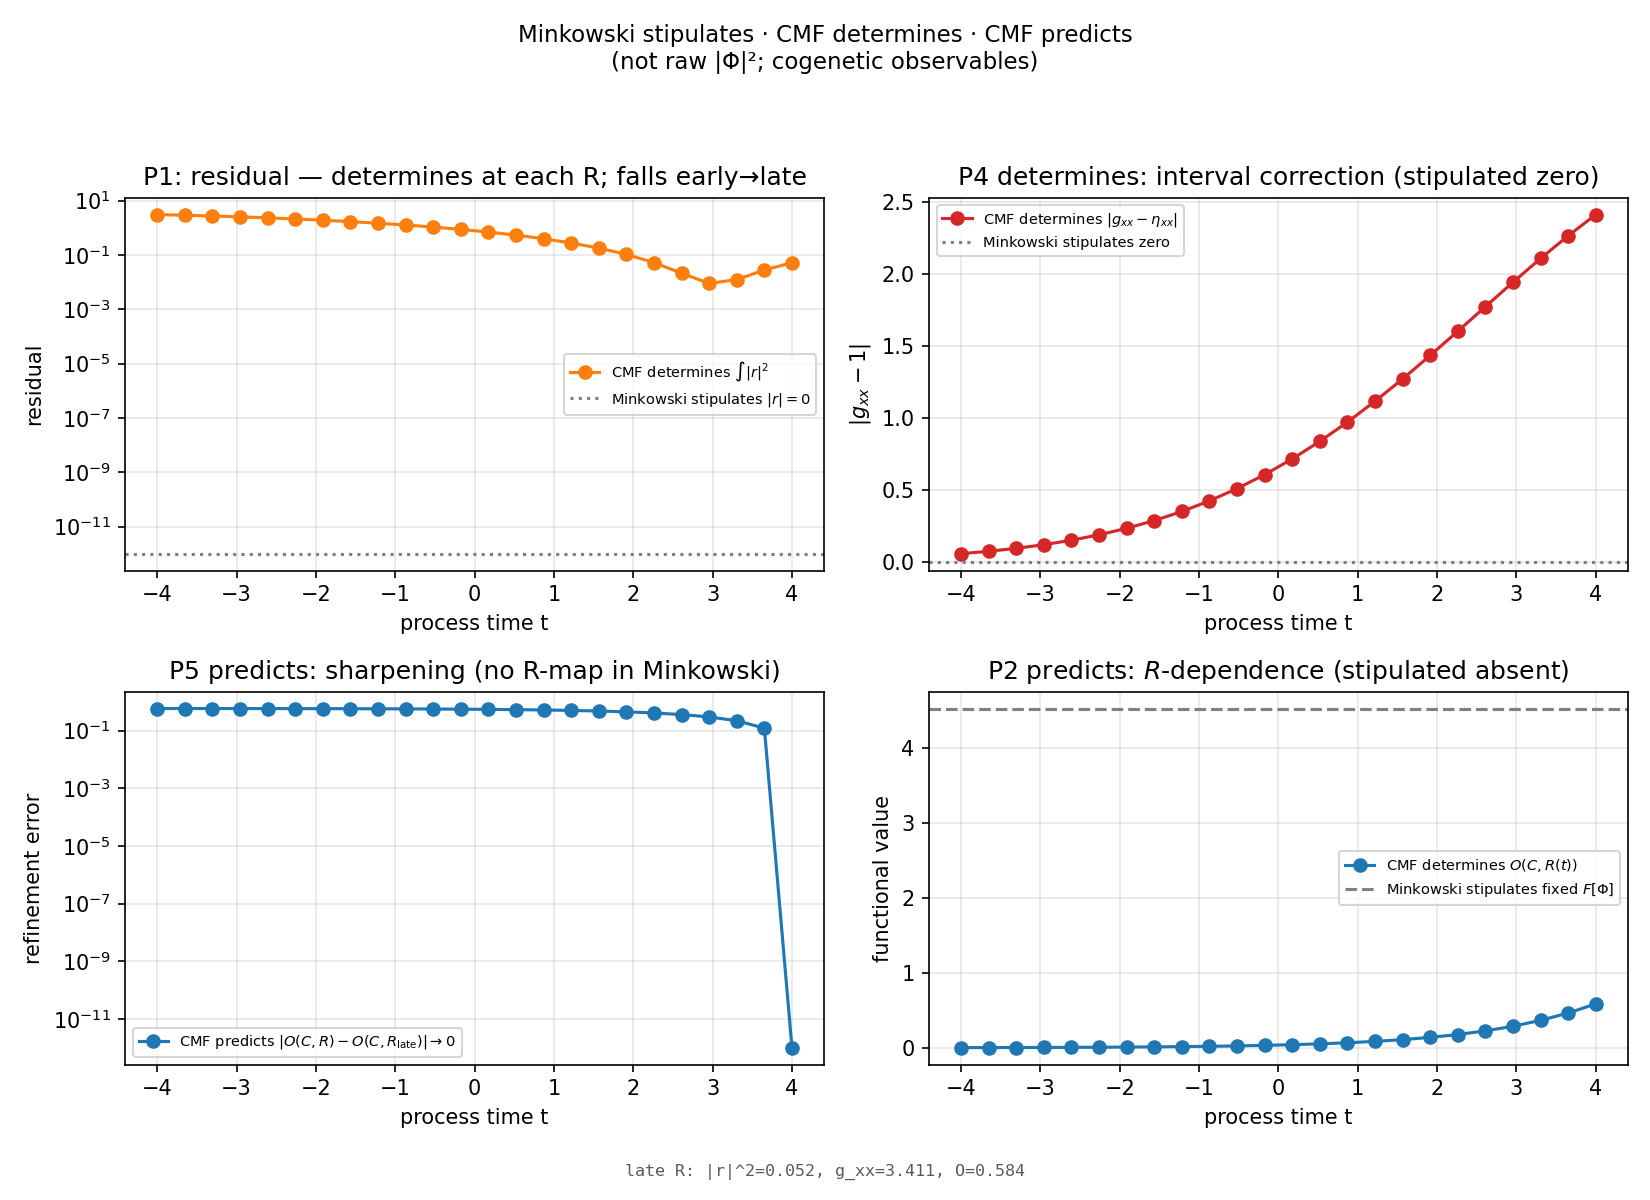
\includegraphics[width=0.88\linewidth]{output/predictions.png}
  \caption{Stipulations vs.\ determination vs.\ prediction (\texttt{python demo.py}). Top row: CMF \emph{determines} residual and interval correction; Minkowski \emph{stipulates} both zero. Bottom row: CMF \emph{predicts} refinement and $R$-dependence; Minkowski \emph{stipulates} no $R$-map.}
  \label{fig:predictions}
\end{figure}

\section{Worked example: satellite point detector}

\paragraph{Setup.}
\begin{itemize}[noitemsep]
  \item Observer (satellite) at altitude $x=-7$, target at surface $x=0$.
  \item Environmental density: $\rho_{\mathrm{env}}(x) = \exp(-|x|/H)$ (exponential atmosphere).
  \item Context: $C = \hat{n}\cdot\nabla\rho_{\mathrm{env}}$ along the throughline \eqref{eq:context-gradient}.
  \item Process field $\Ph$: Gaussian target packet on the surface.
\end{itemize}

\paragraph{Results (reference implementation).}
At early process time ($R=t=-4$), projection is coarse: $|r_{C,R}|^2 \approx 3.1$ and $g_{xx}\approx 1.06$ at the target (cf.\ Minkowski $\eta_{xx}=1$). At late process time ($R=t=4$), the residual falls to $|r_{C,R}|^2 \approx 0.05$; refinement error $|O(C,R)-O(C,R_{\mathrm{late}})|$ approaches zero. The process functional $F[\Ph;C,R(t)]$ shifts from $\approx 0.002$ to $\approx 0.58$ while a fixed functional $F[\Ph]=\int|\Ph|^2\,d\mu \approx 4.52$ is unchanged at all $R$---$C$ and $R$ play no role inside the bolted-on map. Vacuum regions carry $g_{xx}=1$ throughout; flat Minkowski is the valid zeroth-order description where $|r_{C,R}|$ is negligible, not necessarily where the resolved process field has structure.

\begin{figure}[htbp]
  \centering
  \begin{subfigure}[t]{0.32\textwidth}
    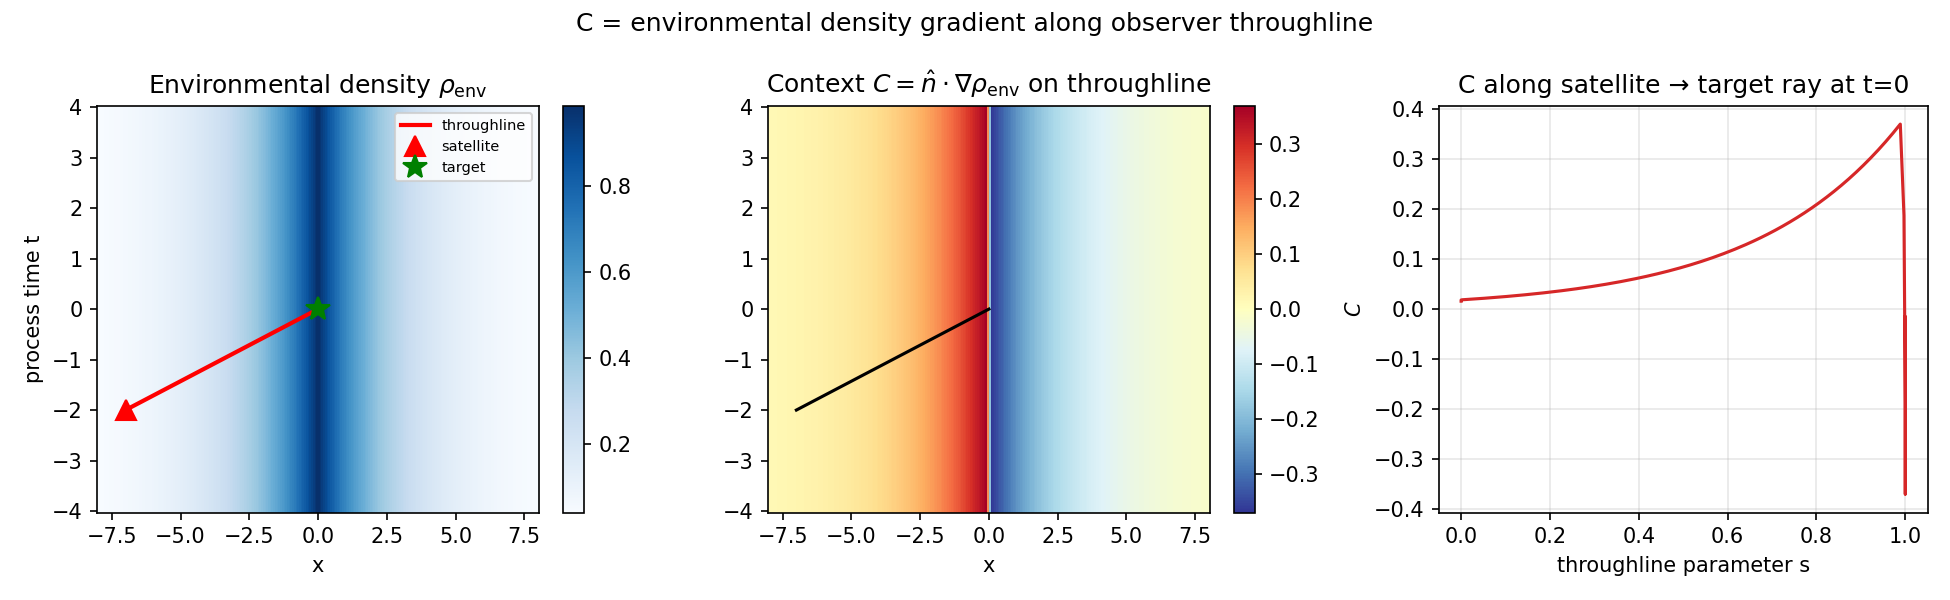
\includegraphics[width=\linewidth]{output/throughline.png}
    \caption{Context $C$ along throughline}
  \end{subfigure}\hfill
  \begin{subfigure}[t]{0.32\textwidth}
    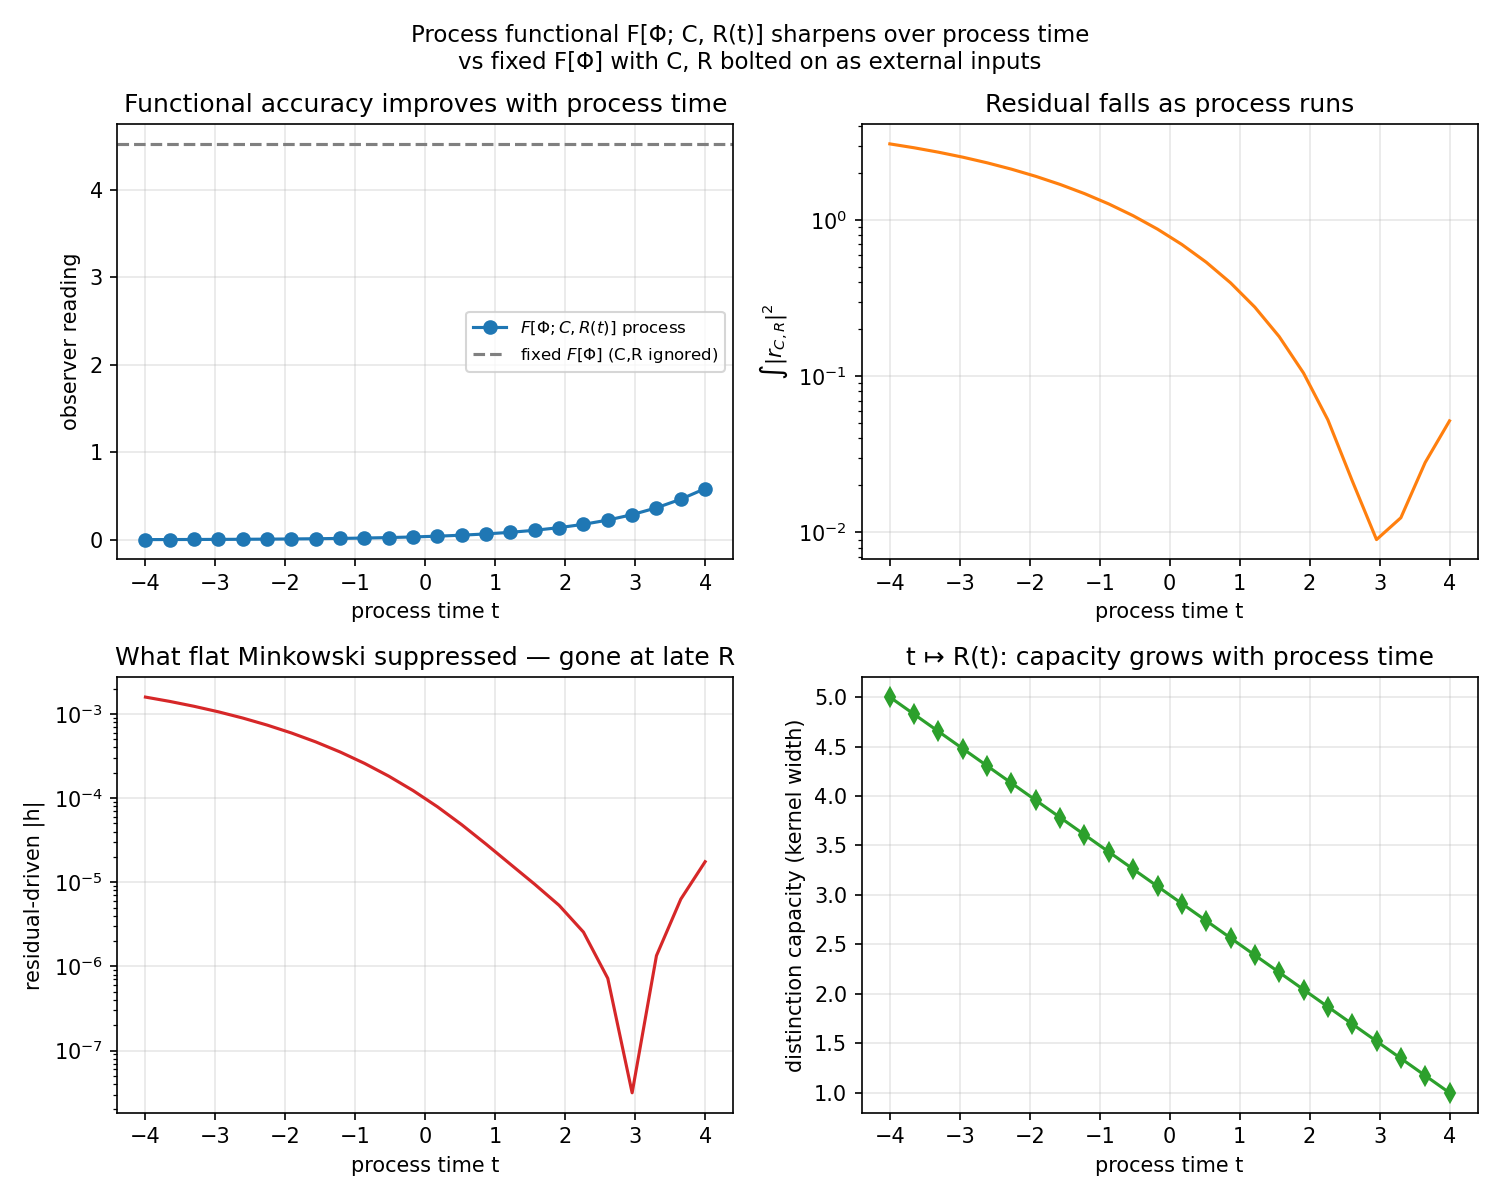
\includegraphics[width=\linewidth]{output/process.png}
    \caption{Process vs.\ bolted-on functional}
  \end{subfigure}\hfill
  \begin{subfigure}[t]{0.32\textwidth}
    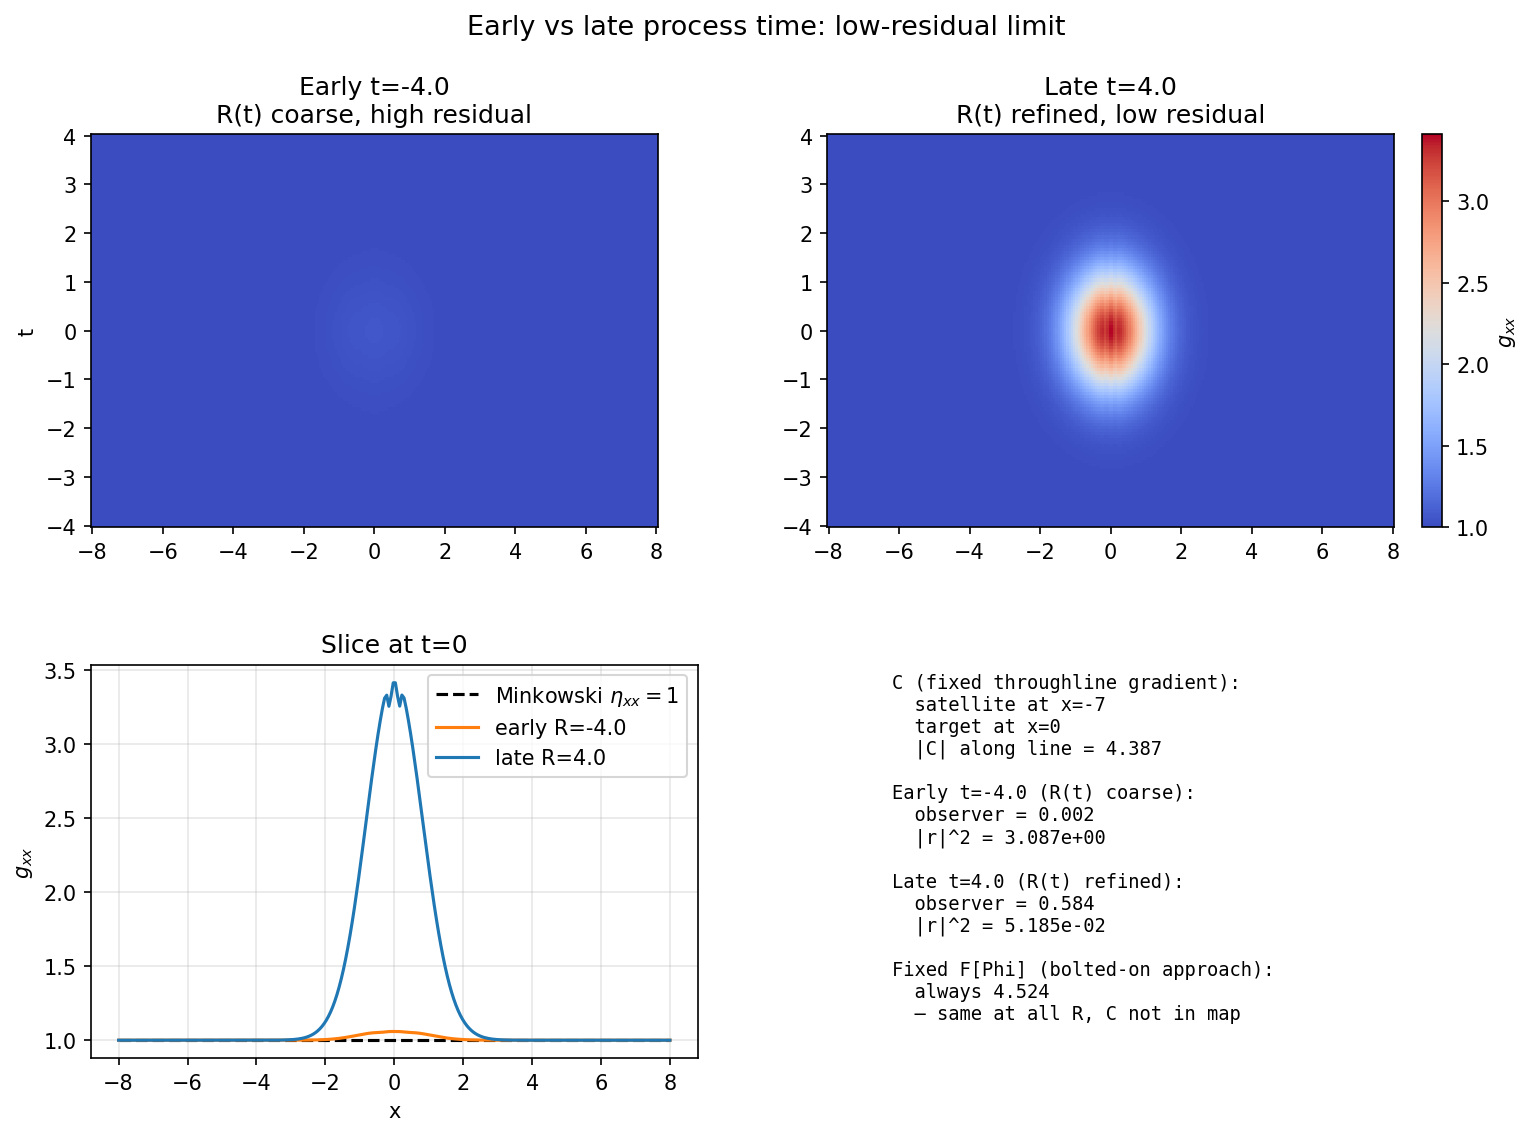
\includegraphics[width=\linewidth]{output/comparison.png}
    \caption{Early vs.\ late process time}
  \end{subfigure}
  \caption{Reference implementation figures (\texttt{python demo.py}).}
  \label{fig:demo}
\end{figure}

\section{Reference implementation}

\begin{table}[h]
  \centering
  \caption{Release artefacts.}
  \label{tab:files}
  \begin{tabular}{@{}ll@{}}
    \toprule
    File & Role \\
    \midrule
    \texttt{cmf.tex} & LaTeX source (this document) \\
    \texttt{cmf.pdf} & Compiled release PDF \\
    \texttt{model.py} & Core CMF: $C$ as throughline gradient; $t \mapsto R(t)$ resolution state \\
    \texttt{demo.py} & Satellite demonstration; generates release figures \\
    \texttt{requirements.txt} & \texttt{numpy}, \texttt{scipy}, \texttt{matplotlib} \\
    \texttt{README.md}, \texttt{LICENSE} & Release metadata \\
    \texttt{output/} & Demonstration figures \\
    \bottomrule
  \end{tabular}
\end{table}

\section{Relation to deeper process geometry}

The \emph{Cogenesis} construction~\cite{petrik2026cogenesis} gives a deeper form:
\begin{equation}
  d\Sigma^2_{C,R} = \langle \delta_{C,R}\Ph,\, G_{C,R}[\Ph]\, \delta_{C,R}\Ph \rangle + r_\Sigma
\end{equation}
with classical metric geometry recovered by projection:
\begin{equation}
  ds^2 = \pi_{\mathrm{geom}}(d\Sigma^2_{C,R})
\end{equation}
CMF represents this projection as an effective metric family $g^{C,R}_{\mu\nu}$---calculus-safe, without pretending the full $d\Sigma^2$ has been captured by $ds^2$ alone. Where a single shared causal cone and metric already unify sectors at the calculus level~\cite{petrik2025omqg}, CMF specifies how flat $\eta$ arises as the low-residual projection of that deeper process under declared context and process time.

\section{Conclusion}

CMF keeps the Minkowski projection calculus without reifying it---against the process calculus that carries $C$, $R(t)$, and residual:
\begin{itemize}[noitemsep]
  \item \textbf{Same machinery}---manifolds, tensors, kernels, PDEs, variational methods.
  \item \textbf{Same simplification exit}---flat $\eta$ when $|r_{C,R}|$ is negligible and the accounting task allows it.
  \item \textbf{No reification}---$C$ and $R(t)$ inside the functional; process time indexes resolution, not a fused spacetime ontology.
  \item \textbf{Relational dynamics}---events, intervals, and metrics from observation process, not primitive points on $\M$.
\end{itemize}

The upgrade is not heavier machinery. It is refusing to mistake projected bookkeeping for ground.

\vspace{1em}
\noindent
{\small
\begin{equation*}
  \boxed{
  \begin{aligned}
    \text{Reified:}\quad &( \M, \eta_{\mu\nu} ) && \text{as primitive spacetime} \\[4pt]
    \text{CMF:}\quad &( \M, \eta_{\mu\nu}, \Ph, \Pi_{C,R}, r_{C,R}, g^{C,R}_{\mu\nu} ) \\[4pt]
    &&& \text{flat $\eta$ when $|r_{C,R}| \to 0$---utilitarian simplification, not ontology.}
  \end{aligned}
  }
\end{equation*}
}

\begin{thebibliography}{9}

\bibitem{petrik2026cogenesis}
M.~Petrik and Militant.AI,
\textit{Cogenesis},
Zenodo, 2026.
\href{https://doi.org/10.5281/zenodo.20539999}{doi:10.5281/zenodo.20539999}

\bibitem{petrik2025omqg}
M.~Petrik and Militant.AI,
\textit{One-Metric Quantum Gravity: Unifying SR, GR, and QM with a Shared Causal Cone},
Zenodo, 2025.
\href{https://doi.org/10.5281/zenodo.17731104}{doi:10.5281/zenodo.17731104}

\end{thebibliography}

\end{document}
